\documentclass[
%% TIKZ_CLASSOPTION %%
tikz
]{standalone}
\usepackage{amsmath}
\usetikzlibrary{matrix}
%% EXTRA_TIKZ_PREAMBLE_CODE %%
\begin{document}
%% TIKZ_CODE %%
\usetikzlibrary{calc}
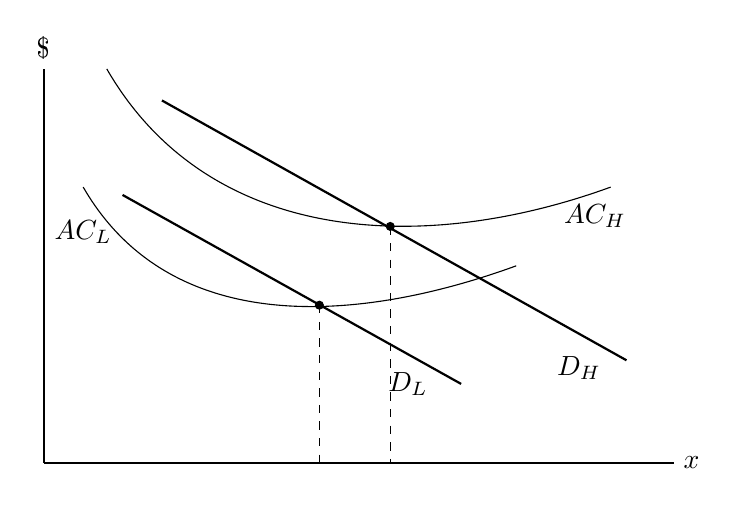
\begin{tikzpicture}[scale=1]
\draw [thick] (0,0) -- (8,0);
\draw [thick] (0,0) -- (0,5);
\node [right] at (8,0) {$x$};
\node [above] at (0,5) {\$};
\draw [thick] (1.5,4.6) -- (7.4,1.3);
\node [left] at (7.2,1.2) {$D_{H}$};
\draw [thick] (1,3.4) -- (5.3,1);
\node [left] at (5,1) {$D_{L}$};
\draw (.5,3.5) to [out=300,in=200] (6,2.5);
\node [below] at (.5,3.2) {$AC_{L}$};
\draw (.8,5) to [out=300,in=200] (7.2,3.5);
\node [below] at (7,3.4) {$AC_{H}$};
\draw[dashed](3.5,2)--(3.5,0);
\draw [fill] (3.5,2) circle [radius =0.05];
\draw[dashed](4.4,3)--(4.4,0);
\draw [fill] (4.4,3) circle [radius =0.05];
\end{tikzpicture}

\end{document}
